\documentclass{article}

\usepackage{Vor2018skil}

\title{Tölvunarfræði 2, \semester \\ Skilaverkefni 0}
\author{}

\begin{document}
\maketitle
\hypersetup{pdftitle={Tölvunarfræði 2 - Skilaverkefni 0}}

Skila skal þessum verkefnum á \href{https://gradescope.com/courses/14122}{Gradescope}.

Þegar forriti er skilað inn til yfirferðar er mikilvægt að láta \textbf{niðurstöðurnar fylgja}. Öllum forritskóða skal skila framsettum með jafnbilaletri. Hann þarf að vera afritanlegur úr .pdf skjalinu. Vönduð framsetning og læsilegur kóði er hluti af verkefninu.

\section{Vísir að uppsetningarleiðbeiningum fyrir GCC}

Stærsti hluti þessa verkefnis er að setja upp starfshæfan C++ þýðanda.

Tölvuuppsetningar eru álíka mismunandi og þær eru margar. Því er erfitt að gefa almennar upplýsingar um hvernig best sé að setja upp C++ þýðandann.

Hér má finna leiðbeiningastúfa fyrir helstu PC-stýrikerfin.

\subsection{Þýðandi}

\subsubsection{Microsoft Windows}

Nokkrir valkostir standa til boða á Windows.

\paragraph{Mingw} Hægt er að nota GCC beint á Windows-skipanalínunni (cmd.exe) með því að setja upp \href{http://mingw-w64.org}{mingw-w64}. Einnig þarf að gæta að því að GCC sé í í PATH.

\paragraph{Cygwin} Hægt er að nota \href{https://www.cygwin.com/}{Cygwin} til að herma eftir Linux-skipanalínu. Við uppsetningu þarf þá að velja \texttt{gcc-core} og \texttt{gcc-g++} pakkana.

\paragraph{Linux Subsystem} Windows 10 býður upp á að keyra Linux-skipanalínuforrit í gegnum \href{https://docs.microsoft.com/en-us/windows/wsl/install-win10}{Linux Subsystem}. Sé Ubuntu valið má fylgja Linux-leiðbeiningunum að neðan.

\subsubsection{Mac OS X}

Setja þarf upp xcode command line tools. Það má gera með því að keyra skipunina 

\texttt{xcode-select --install}

í Terminal.

\subsubsection{Linux}

Líklegt er að GCC-þýðandinn sé foruppsettur. Sé svo ekki er hægt að setja hann upp í gegnum pakkakerfi útgáfunnar.

Á Ubuntu og ættingjum þess má setja þýðandann upp með því að keyra

\texttt{sudo apt-get install build-essential}

á skipanalínu.

\subsubsection{Engin fjárans uppsetning}

Líklegt er að til sé ``online'' C++ þýðandi sem dugar fyrir námskeiðið. Ég þekki engan sem hægt er að mæla með. Helsta krafan sem ekki er sjálfgefin er að hann geti lesið vandræðalaust inn af staðalinntaki.

Einnig er hægt að leysa a.m.k. fyrsta verkefnið með því að nota ssh-tengingu við Heklu (hekla.rhi.hi.is) og vinna verkefnið þar. Skrár á Heklu eru tengdar við HÍ-heimasvæðið ykkar, sem getur auðveldað vinnslu. Þýðandinn sem þar er uppsettur er þó kominn nokkuð til ára sinna og gæti valdið vandræðum.

\subsection{Ritill}

Allir almennir forritunarritlar duga í þessu námskeiði fyrir C++ og Java.

Þeim nemendum sem ekki eiga sinn uppáhalds ritil er bent á að \href{https://code.visualstudio.com/}{Visual Studio Code} er opinn og gjaldfrjáls ritill sem vitað er að virkar á helstu stýrikerfum. Sjá \href{https://code.visualstudio.com/docs/languages/cpp}{VS Code C++ leiðbeiningar}.

\begin{figure}[hb]
    \caption{C++ kóði í Visual Studio Code}
    \begin{center}
        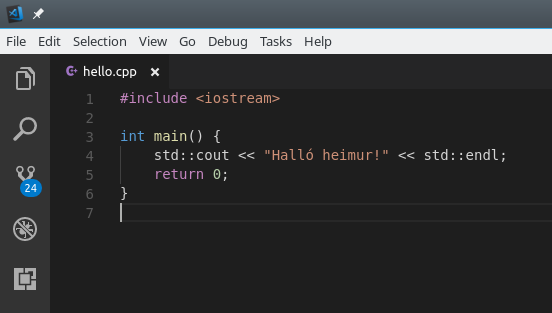
\includegraphics[width=\textwidth]{vscode-hello-world}
    \end{center}
\end{figure}

\newpage

\section{Verkefnið sjálft}

Hér eru verkefnin tvö sem skila á inn á Gradescope.

\question

Takið \href{https://raw.githubusercontent.com/Ernir/kennsluefni/master/T2/Code/w1/hello.cpp}{``Halló Heimur'' C++ forritið úr fyrirlestri}, þýðið það og keyrið.

Þegar það hefur verið keyrt skuluð þið bæta \texttt{``, ég heiti <nafn>!''} aftan á setninguna sem skrifuð er út. Skilið skjáskoti (e. \emph{screenshot}) af keyrslunni sem er ekki eins og skjáskot annars nemanda.

Dæmi sést á mynd \ref{hello-ernir}.
\begin{figure}[h!]
    \label{hello-ernir}
    \begin{center}
        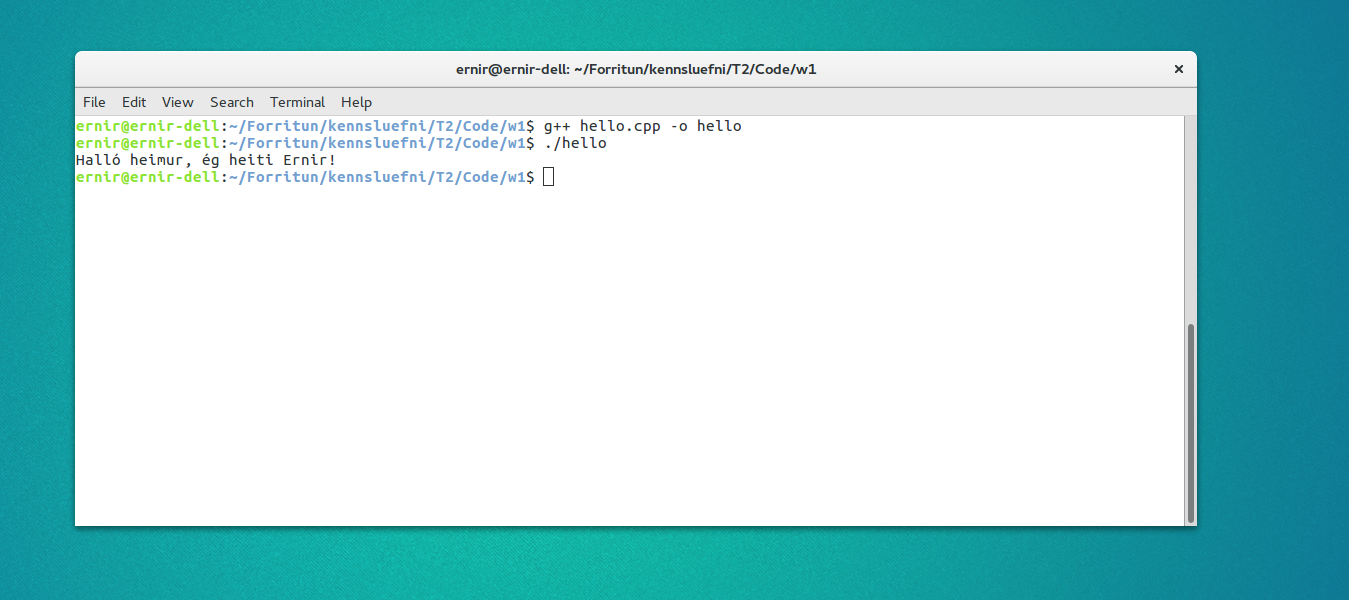
\includegraphics[width=\textwidth]{hello-ernir}
    \end{center}
\end{figure}

\question

Skrifið C++ forrit sem les inn tölur af staðalinntaki. Þegar innlestrinum er lokið skal forritið skrifa út summu þeirra og meðaltal.

Dæmi:
\begin{minted}{bash}
$ g++ average.cpp -o average && ./average
2
3
4
2
Summa talnanna er 11
Meðaltal talnanna er 2.75    
\end{minted}

\vfill

\includegraphics[width=0.5\linewidth]{hi-von-logo}
\end{document}